\documentclass[sigconf,anonymous,review]{acmart}
\AtBeginDocument{\providecommand\BibTeX{{\BibTeX}}}
\setcopyright{none}
\settopmatter{printacmref=false,printccs=true,printfolios=true}
\renewcommand\footnotetextcopyrightpermission[1]{}
\acmConference[KDD '27]{The 33rd ACM SIGKDD Conference on Knowledge Discovery and Data Mining}{August 1--5, 2027}{San Jose, California, USA}
\acmYear{2027}
\copyrightyear{2027}
\usepackage{mathtools}
\usepackage{booktabs}
\usepackage{enumitem}
\usepackage{graphicx}
\usepackage{tabularx}
\usepackage{microtype}
\usepackage{url}
\usepackage{xurl}
\setlength{\emergencystretch}{1em}
\usepackage{tikz}
\usetikzlibrary{arrows.meta,positioning,calc,fit}
\newcommand{\F}{\mathcal F}
\newcommand{\T}{\mathcal T}
\newcommand{\R}{\mathcal R}
\newcommand{\ind}{\mathbb I}
\newcommand{\methodname}{\textsc{EventFrontier}}
\newtheorem{proposition}{Proposition}
\newtheorem{lemma}{Lemma}
\newtheorem{theorem}{Theorem}
\title{EventFrontier: Aggregate Identification from Logs with Hidden Event Membership and Coarsened Time}
\begin{document}
\begin{abstract}
Event logs can preserve individual participations while suppressing event
identifiers and coarsening timestamps. Aggregate queries about shared events
then depend on both a hidden partition and a common time realization.
Existing uncertain-linkage bounds motivate our approach, but pairwise
compatibility alone need not describe a realizable temporal event.
We introduce \methodname, a conditional identification framework for
positive-overlap-connected events with bounded simultaneous occupancy.
Sequential turnover permits event membership to exceed capacity; uncertain
timestamps must be completed jointly. For exact intervals, fixed root and span,
and additive row weights, segment-coverage and boundary-bridge constraints
yield an integral LP pricing oracle. We embed it in a nonintegral event-column
master and branch-and-price for support maximization; uncertain-time models
retain explicit feasibility and unresolved statuses. In 3,000 controlled
instances, a feasible point rule makes 17.4--19.0\% threshold errors, all
flagged when the true world is admissible. On annotated pedestrian dyads, a
pilot-selected support retains 81/82 follow-up worlds but certifies only
29/246 decisions. A Chicago pair benchmark numerically closes 2,744 data-complete endpoint
pairs across 23 eligible pilot windows; a separate 96-window follow-up
remains incomplete. NYC yields 125 witness-certified ambiguous cells out of
126, but a fixed-input structural audit finds no endpoint change in 24
comparable model comparisons. The evidence supports conditional ambiguity and
bounded-scale computation while leaving the public-data advantage of general
ordered-event structure unresolved.
\end{abstract}
\ccsdesc[500]{Information systems~Data provenance}
\ccsdesc[500]{Information systems~Data integration}
\ccsdesc[500]{Theory of computation~Mathematical optimization}
\ccsdesc[300]{Computing methodologies~Structured outputs}
\keywords{partial identification, temporal event logs, hidden event membership, interval graphs, branch-and-price}
\maketitle
\section{Introduction}

Public event logs can reveal every recorded participation while suppressing
the identifier that joins participations into a shared event. A shared-trip
record, for example, may expose departure time, duration, and destination but
omit its vehicle-run key. The analyst can count trips directly; measuring
within-event composition or comparing outcomes across possible co-participants
requires a relation that the release does not supply. A reproducible point
reconstruction selects one explanation of these rows, but its aggregate answer
need not survive other explanations allowed by the same observations.

Aggregate bounds under uncertain linkage are an established response to this
problem \citep{turkcapar2023aggregate,hua2012aggregate}. Our focus is the
additional structure of \emph{temporal events}: participants enter and leave,
capacity limits simultaneous occupancy rather than total membership, and
released timestamps can themselves be uncertain. A two-seat event can contain
three sequential participants even when the first and last never coexist.
Conversely, two individually possible overlaps may require incompatible
realizations of a shared participant's time. Pairwise candidate compatibility
therefore does not establish joint temporal-event feasibility.

The resulting question is specific:
\begin{quote}
Which aggregate conclusions hold across all event partitions that admit one
common timestamp completion satisfying the declared connectivity and
simultaneous-capacity constraints?
\end{quote}
We call the input \emph{relation-incomplete}; row completeness, when assumed,
is relative to a declared candidate universe and observation protocol. It is
not a guarantee that every operational participant appears in a public extract.

\methodname{} represents a feasible world by a timestamp completion and a
partition of selected rows into positive-overlap-connected events. Required
core rows define the cohort, while optional boundary rows can complete its
events without being forced into the cohort themselves. Aggregate extrema
describe the conclusions supported by this model. They are conditional
identified bounds, not confidence intervals or recovered event identities.
The model deliberately omits unobserved routing and provider rules; a
temporally feasible world need not be operationally realizable in every domain.

The computational challenge is the implicit family of possible events.
Even with exact timestamps, optimizing each event independently is insufficient:
events compete for the same rows. We exploit a local interval structure and
retain an integer search for their global coupling. Set-valued timestamps are
handled separately through joint feasibility, rather than assuming that a
polynomial exact-time subproblem also solves uncertain-time instances.

Our contributions are threefold.
\begin{enumerate}[leftmargin=*,itemsep=2pt,topsep=3pt]
\item \textbf{A precise event-level identification model.} We combine required
and optional rows, sequential membership, simultaneous occupancy, and joint
timestamp completion. Separation examples show why event cardinality, pairwise
compatibility, and outer time envelopes cannot substitute for these conditions.
Support nesting and threshold certification specify the resulting guarantee;
they are consequences of possible-world semantics, not new general principles.
\item \textbf{An integral local optimization primitive.} With exact intervals,
a fixed root and span, and additive row weights, interleaved segment-coverage
and boundary-bridge constraints preserve the consecutive-ones structure. The
resulting integral LP prices a single event. We integrate this primitive into
Dantzig--Wolfe decomposition and branch-and-price for support maximization,
with a nonintegral master and explicit bounds when search is incomplete.
\item \textbf{An audit separating three evidentiary questions.} Controlled
ordered-event instances check optimization and decision logic. Annotated
pedestrian dyads test whether geometric candidate rules retain a real relation.
Public Chicago and NYC records test conditional ambiguity and computational
coverage. No experiment is used as evidence for a different layer's claim.
\end{enumerate}

In 3,000 controlled instances, a feasible temporal point rule has
17.4--19.0\% threshold error; the frontier flags all observed errors when truth
is admissible. This is a validation implication of coverage. More informative
is its failure boundary: candidate truncation retains about 84\% of true
members but only 31--33\% of complete true worlds. In the annotated dyad
audit, a pilot-selected support retains 81/82 follow-up worlds yet certifies
only 29/246 decisions. Coverage, sparsity, and decision informativeness are
different properties.

The public results also delimit the contribution. The completed Chicago
24-window pilot has 23 eligible windows and 2,744 certified numerical endpoint
pairs, with 686 pairs excluded for missing public values. Its 96-window
follow-up is incomplete. NYC has 125 witness-certified ambiguous decisions
among 126 outcome--capacity cells, while a separate 18-cell support-maximization
lattice closes through 16 cores and 48 buffers. A fixed-input structural audit
finds \emph{no} endpoint change in 24 comparable restricted-versus-ordered
comparisons. Thus public-data evidence currently supports conditional ambiguity
and bounded-scale computation; it does not yet establish an empirical advantage
from the general event model. This distinction determines both what the paper
claims and what further evidence is needed.

\section{Related Work}
\label{sec:related}

\paragraph{Aggregate uncertainty from unresolved relationships.}
Resolution-aware query answering retains unresolved entities and computes
aggregate bounds without requiring probabilities over resolutions
\citep{sismanis2009resolution}. Probabilistic linkage supports aggregate
queries \citep{hua2012aggregate}; constrained probabilistic similarity joins
likewise define one-to-one, one-to-many, and many-to-many matching worlds and
evaluate aggregates over them \citep{chen2019constrained}. Bayesian linkage
represents entire compatible matchings and quantifies their uncertainty
\citep{sadinle2017linkage}. Our closest optimization comparator,
\citet{turkcapar2023aggregate}, computes aggregate ranges over
candidate-constrained one-to-many table integrations via graph matching. It
also studies false-negative candidates and failure to cover the true
aggregate. Thus possible-world aggregation, matching constraints, extremal
bounds, and candidate-omission risk are not new here.

The narrow distinction is the latent world being quantified over. A matching
selects links; our world partitions rows into variable-cardinality temporal
events. Each event must admit one common timestamp completion, connected
positive overlap, and bounded occupancy at every instant. Consequently,
membership can exceed capacity through sequential turnover, while individually
compatible links may be jointly unrealizable. These are object-level
constraints rather than a new semantics for uncertain aggregation.

\paragraph{Possible worlds, repairs, and sensitivity.}
Range-consistent query answering optimizes aggregates across legal database
repairs, with tractability results for query rewriting under primary-key
violations \citep{elkhalfioui2024range,elkhalfioui2026upper}.
Attribute-uncertain databases propagate value bounds through relational
queries \citep{feng2021audb}. EventFrontier adopts the same general principle
of quantifying over admissible worlds; its contribution concerns a temporal
event family, rather than a new semantics for uncertain data. Query resilience
studies the smallest input deletion that makes a Boolean query false
\citep{freire2015resilience}. Our omission budgets instead parameterize
candidate support for latent relationships. We report sensitivity within this
declared family, without claiming a new general notion of robustness or an
unconditional coverage guarantee.

\paragraph{Interval optimization and decomposition.}
Interval scheduling already admits structured pricing, column generation,
and branch-and-price. In particular, \citet{muir2023interval} partition fixed
interval jobs under economies-of-scale costs, giving polynomial pricing for
the max-weight case and pseudo-polynomial pricing for a broader class.
Their schedules forbid simultaneous jobs on the same machine; our events
require positive-overlap connectivity while limiting occupancy. Our local
result jointly encodes segment coverage, boundary bridges, capacity, and
fixed membership in a consecutive-ones formulation. For fixed exact times,
root, span, and additive weights, this yields an integral event-pricing LP.
Total unimodularity and decomposition are established tools; the specific
claim is their applicability to this connected event formulation.
The coupled master can remain fractional, and branch-compatible pricing may
require exponentially many cases. We make no polynomial-time claim for the
full partition problem or for arbitrary set-valued timestamps.

\paragraph{Mobility as an observation setting.}
Shareability networks and trip--vehicle assignment optimize prospective
allocations \citep{santi2014shareability,alonsomora2017ondemand}.
Studies of public ride-hailing data predict sharing outcomes or construct
proxy groups \citep{taiebat2022sharing,sebtichen2026hidden}.
Our application instead asks which retrospective aggregates are compatible
with released rows after event identifiers and time precision are removed.
The public audits establish conditional ranges, not recovery of actual
vehicle assignments or evidence of social interaction. Chicago and ATR
dyads test the matching special case and candidate-support validity; evidence
for the general temporal-event contribution must additionally exercise
sequential membership and joint timestamp feasibility.

\section{Identification over Hidden Event Worlds}
\label{sec:model}

\paragraph{Records, time supports, and boundary rows.}
The observed universe is a finite disjoint union $V=C_0\cup B_0$.
Core rows $C_0$ define a cohort declared to consist of shared-event
participants. Buffer rows $B_0$ are possible members of events crossing its
observation boundary. Every core must be assigned; buffers may remain unused.
These roles and the candidate universe are assumptions of the audit, not
relations recovered by the optimization.

Row $i$ has public attributes and a nonempty timestamp support
$\T_i\subseteq\{(s,e):s<e\}$. A completion chooses
$t_i=(s_i,e_i)\in\T_i$, yielding the half-open interval $I_i=[s_i,e_i)$.
Exact timestamps give singleton supports. Positive overlap means
$|I_i\cap I_j|>0$; endpoint touching does not count.

\paragraph{Events and worlds.}
At simultaneous capacity $C$, an event is a subset $R\subseteq V$ containing
at least two rows and one core, with a connected positive-overlap graph and
\begin{equation}
 \max_u\sum_{i\in R}\ind\{u\in I_i\}\le C.
 \label{eq:capacity}
\end{equation}
Capacity limits concurrent participation. It does not limit the total number
of event members: sequential entry and exit permit $|R|>C$
(Figure~\ref{fig:chain}). These constraints define a temporal event model;
they do not establish a physically realized vehicle route.

A world $F=(t,\Pi)$ comprises one completion and a collection of disjoint
feasible events. Every core belongs to exactly one event, and each buffer
belongs to at most one. Let $q(F)$ count selected buffers and define
\[
 \F(\T,C,q)=\{F:q(F)=q\},\qquad
 Q(\T,C)=\{q:\F(\T,C,q)\ne\varnothing\}.
\]
Write $M(\T,C)=\max Q(\T,C)$ when $Q$ is nonempty. Feasibility requires a
\emph{common} completion for all relationships within each event.

\begin{proposition}[Pairwise possibility does not imply event feasibility]
\label{prop:jointcompletion}
Let $I_A=[0,1)$, $I_C=[3,4)$, and $I_B=[s,s+1)$ with $s\in[0,3]$.
Pairs $AB$ and $BC$ can each overlap under some completion, but no completion
makes $\{A,B,C\}$ a connected event, even at capacity two.
\end{proposition}

Indeed, the two overlaps require $s<1$ and $s>2$, respectively.
The proposition isolates a modeling distinction: a graph of individually
possible edges loses the joint time constraints. It is not a general
inexpressibility claim about uncertain-database formalisms.

\paragraph{Aggregate identification.}
Let $H(F)$ be an event-label-invariant function of public attributes and the
partition, defined on the worlds being compared. Examples include selected
buffer means, within-event dispersion, and event count per core.
For nonempty $\F(\T,C,q)$,
\begin{equation}
 \underline H(\T,C,q)=\min_{F\in\F(\T,C,q)}H(F),\quad
 \overline H(\T,C,q)=\max_{F\in\F(\T,C,q)}H(F).
 \label{eq:endpoints}
\end{equation}
There are finitely many partitions, so these extrema are attained for the
stated class of $H$. This definition does not imply an efficient algorithm
for every aggregate. A threshold rule $\ind\{H\ge\eta\}$ is certified positive
when $\underline H\ge\eta$, negative when $\overline H<\eta$, and ambiguous
otherwise. Correctness is conditional on the true world belonging to $\F$.

\begin{proposition}[Support and capacity nesting]
\label{prop:nesting}
If $\T_i\subseteq\T'_i$ for each row and $C\le C'$, then
$\F(\T,C,q)\subseteq\F(\T',C',q)$ for every $q$. Consequently $Q$ expands
and $M$ cannot decrease whenever it is defined. At a common feasible $q$,
\[
 \underline H(\T',C',q)\le\underline H(\T,C,q),\qquad
 \overline H(\T',C',q)\ge\overline H(\T,C,q).
\]
\end{proposition}

This is set-inclusion reasoning, not an additional optimization result.
Evaluating each capacity at its own $q=M(\T,C)$ changes the conditioning
population, so those outcome ranges need not nest.

\begin{figure}[t]
\centering
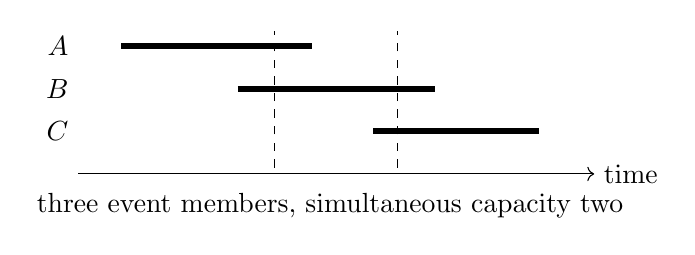
\begin{tikzpicture}[x=0.78cm,y=0.54cm]
\draw[->] (0,0) -- (8.4,0) node[right]{time};
\foreach \y/\lab in {3/A,2/B,1/C}{
  \node[left] at (0,\y) {$\lab$};
}
\draw[line width=2.2pt] (0.7,3) -- (3.8,3);
\draw[line width=2.2pt] (2.6,2) -- (5.8,2);
\draw[line width=2.2pt] (4.8,1) -- (7.5,1);
\draw[dashed] (3.2,0.15) -- (3.2,3.35);
\draw[dashed] (5.2,0.15) -- (5.2,3.35);
\node[align=center] at (4.1,-0.75) {three event members, simultaneous capacity two};
\end{tikzpicture}
\caption{A feasible fixed-time event can be an overlap chain. This differs
from both a clique and the two-member restriction $K=2$.}
\Description{Three intervals form a positive-overlap chain, with at most two
active simultaneously.}
\label{fig:chain}
\end{figure}

\section{Structure-Exploiting Optimization}
\label{sec:algorithm}

\subsection{The declared $K=2$ special case}
If every event must contain exactly two rows, the world reduces to a
core-cover matching: every core has degree one, every buffer has degree at most
one, and buffer--buffer edges are excluded. Pair-additive queries become
weighted matching objectives. This is the Chicago benchmark and a useful
lower-complexity special case, but it cannot represent sequential
higher-cardinality events such as Figure~\ref{fig:chain}.

\begin{theorem}[$K=2$ core-cover matching equivalence]
\label{thm:k2matching}
Let $G=(C_0\cup B_0,E)$ contain every admissible two-row event incident to at
least one core row, with no buffer--buffer edge.  Feasible $K=2$ worlds are in
bijection with matchings in $G$ that saturate every vertex of $C_0$.  Under the
bijection, every pair-additive aggregate equals the corresponding edge-weight
sum.  Hence both frontier endpoints are exactly minimum- and maximum-weight
core-saturating matching problems.
\end{theorem}

\paragraph{Proof.}
Map each two-row event in a feasible world to its edge.  Disjoint event
membership implies that the selected edges form a matching, and core coverage
implies that every core vertex is saturated.  Conversely, every matching that
saturates $C_0$ defines disjoint two-row events covering each core exactly once;
unmatched buffers are unused.  These maps are inverse.  Pair additivity gives
equality of the world aggregate and selected-edge weight term by term.

The matching representation also localizes the source of a nondegenerate
frontier. For a matching $M$, write $w(M)=\sum_{e\in M}w_e$.

\begin{theorem}[Alternating decomposition of a fixed-cardinality $K=2$ frontier]
\label{thm:k2alternating}
Let $M^-$ and $M^+$ be any minimum- and maximum-weight feasible matchings of
the same cardinality $q>0$. Their symmetric difference is a vertex-disjoint
union $\mathcal A$ of alternating paths and even alternating cycles. Every
cycle contains equally many edges of $M^-$ and $M^+$; every path has edge-count
imbalance in $\{-1,0,1\}$, and these path imbalances sum to zero. Moreover,
\begin{equation}
 \overline H-\underline H
 =\frac{1}{q}\sum_{A\in\mathcal A}
 \left(\sum_{e\in A\cap M^+}w_e-
       \sum_{e\in A\cap M^-}w_e\right).
 \label{eq:alternating-width}
\end{equation}
Thus frontier width is generated by additive exchanges along alternating
components; equal cardinality may couple paths whose individual edge-count
imbalances are nonzero.
\end{theorem}

\paragraph{Proof.}
Every vertex has degree at most two in $M^-\mathbin{\triangle}M^+$ and is
incident to at most one edge of each matching. Each nontrivial connected
component is therefore a path or cycle whose edge colors alternate. A cycle is
even and balanced. An alternating path has equal color counts or one extra edge
of one color. Since $|M^-|=|M^+|=q$, the path imbalances sum to zero. Common
edges cancel from $w(M^+)-w(M^-)$; grouping the remaining terms by component
and dividing by $q$ proves Eq.~\eqref{eq:alternating-width}.

This theorem does not claim that every component can be exchanged alone. A
balanced cycle or path can be, but imbalanced paths must be exchanged in a
cardinality-balanced collection. Nor is the decomposition unique when an
endpoint has multiple optimal witnesses; endpoint values remain unique even
when the returned witness structure is not.

The equivalence also yields a support-omission sensitivity object that does not
depend on released geography.  Fix a declared base edge set $E_0\subseteq E$
and let $d_e=|e\cap C_0|$ for $e\in E\setminus E_0$, with $d_e=0$ otherwise.
For integer $\Gamma\in[0,|C_0|]$, impose
\begin{equation}
  \sum_{e\in E}d_e x_e\leq \Gamma.
  \label{eq:k2omission}
\end{equation}

\begin{proposition}[Nested candidate-omission frontier]
\label{prop:k2omission}
The feasible matching sets in Eq.~\eqref{eq:k2omission} are nested in
$\Gamma$.  At $\Gamma=0$ the set equals the core-saturating matchings using
only $E_0$; at $\Gamma=|C_0|$ it equals the unrestricted set on $E$.
Consequently every lower endpoint is weakly nonincreasing and every upper
endpoint weakly nondecreasing in $\Gamma$.
\end{proposition}

\paragraph{Proof.}
Nesting follows because only the right-hand side increases.  Every omitted
edge has positive core incidence, giving the first endpoint identity.  In any
core-saturating matching, summing $|e\cap C_0|$ over selected edges counts each
core exactly once and therefore equals $|C_0|$; the constraint is redundant at
the second endpoint.  Optimization over nested feasible sets gives the stated
endpoint monotonicity.

\begin{proposition}[When support contraction changes no decision]
\label{prop:k2thresholdcontraction}
Let $E'\subseteq E$ and suppose both fixed-$q$ feasible sets are nonempty. Then
\[
 \underline H_E\leq\underline H_{E'}\leq
 \overline H_{E'}\leq\overline H_E.
\]
For a threshold $\eta$ that is ambiguous under $E$, contraction to $E'$ leaves
the decision ambiguous exactly when
$\underline H_{E'}<\eta\leq\overline H_{E'}$. Hence strict contraction of a
continuous frontier need not improve decision certification.
\end{proposition}

\paragraph{Proof.}
Every feasible matching on $E'$ is feasible on $E$, so minimization over the
smaller set weakly raises the lower endpoint and maximization weakly lowers the
upper endpoint. The threshold rule certifies positive iff the lower endpoint
is at least $\eta$, certifies negative iff the upper endpoint is below $\eta$,
and is ambiguous otherwise, giving the equivalence.

\subsection{A compact connectivity characterization}
Fix exact intervals, a root row $r$, and a candidate span $[a,b)$. Let the
sorted distinct endpoints inside the span induce elementary open segments.
For a selected set containing $r$, positive-overlap connectivity with union
span $[a,b)$ is equivalent to:
\begin{enumerate}[leftmargin=*,itemsep=1pt,topsep=2pt]
\item every elementary segment is covered by at least one selected interval;
\item every internal endpoint boundary is strictly crossed by at least one
selected interval.
\end{enumerate}
The second condition excludes components that only touch at an endpoint.
Capacity adds an upper bound of $C$ to each segment-coverage row.

Interleave segment and boundary rows in temporal order. Each interval column
then contains ones in one consecutive block. This yields the pricing primitive.

\begin{theorem}[Integral rooted single-event oracle]
\label{thm:oracle}
For fixed exact intervals, root $r$, span $[a,b)$, capacity $C$, and additive
row weights, the linear relaxation of the segment-coverage, boundary-bridge,
capacity, root, and forced-companion formulation has an integral optimum.
Hence a minimum- or maximum-weight rooted event can be found by linear
programming. Enumerating observed endpoint spans and, only when needed, one
forced companion gives a polynomial-time exact single-event oracle.
\end{theorem}

\paragraph{Proof sketch.}
The interleaved segment/boundary incidence matrix has the consecutive-ones
property by columns. Signed duplicate rows for lower and upper coverage bounds,
plus identity rows fixing the root and companion, preserve total
unimodularity. The right-hand side is integral, so every extreme point is
integral. Candidate spans need only use observed interval endpoints. Appendix
details and exhaustive small-library comparisons are included in the artifact.

\subsection{Dantzig--Wolfe decomposition}
Let $\R_C$ be all feasible exact-time event columns. For event $R$, let
$b_R=|R\cap B_0|$ and introduce $\lambda_R\ge0$. The full relaxation for maximum
reachable buffer support is
\begin{align}
\max_{\lambda}\quad & \sum_{R\in\R_C}b_R\lambda_R
\label{eq:masterobj}\\
\text{s.t.}\quad
&\sum_{R\ni i}\lambda_R=1 && i\in C_0,\label{eq:coremaster}\\
&\sum_{R\ni j}\lambda_R\le1 && j\in B_0.\label{eq:buffermaster}
\end{align}
Core equalities and buffer inequalities couple otherwise independent event
columns. Given master duals, reduced cost is additive across selected rows, so
Theorem~\ref{thm:oracle} gives exact pricing. A phase-one artificial-core
master establishes feasibility.

\begin{proposition}[Full-master LP certificate]
\label{prop:cg}
If every rooted pricing call is solved exactly and the terminal minimum reduced
cost is nonnegative, the current restricted-master value equals the optimum of
Eqs.~\eqref{eq:masterobj}--\eqref{eq:buffermaster} over all feasible event
columns.
\end{proposition}

Local integrality does not transfer to the coupled master. The appendix gives a
capacity-two instance with
\[
\operatorname{OPT}_{LP}=4>3=\operatorname{OPT}_{IP}.
\]
A restricted integer solve over columns generated only for the root LP can
therefore miss the full integer optimum.

\subsection{Branch-compatible exact integer decomposition}
\label{sec:bp}
We close the support-maximization integer master with branch-and-price. At a
node, optional buffers may be fixed to total usage zero or one. Once row usage
is integral but event columns remain fractional, Ryan--Foster branching chooses
two active rows and creates:
\[
\text{together: both rows have identical membership in every event},\qquad
\text{separate: no event contains both.}
\]
For a priced root, together and separate restrictions are expanded into a
finite set of forced-in/forced-out cases. Each case adds only identity fixes
and variable bounds to the fixed-span formulation, so Theorem~\ref{thm:oracle}
still solves it exactly. The number of cases may grow exponentially with branch
depth; we make no polynomial-time claim for the full integer problem.

\begin{proposition}[Integer certificate]
\label{prop:bp}
Suppose each node relaxation is closed by exact branch-compatible pricing,
every child exhaustively implements its row-usage or Ryan--Foster disjunction,
and the branch queue terminates. Then the incumbent is a globally optimal
integer solution of the full event-column master. If computation stops early,
the best incumbent and largest open-node LP bound form a valid global lower and
upper bound.
\end{proposition}

\paragraph{Justification.}
The two children partition the integer solutions compatible with the parent.
Exact pricing makes each node bound valid for the full, not merely restricted,
column set. Standard branch-and-bound dominance then proves the claim. The
implementation replays every incumbent, records open-node bounds, and never
labels a time-limited cell optimal.

\subsection{Existential timestamp completion}
For set-valued timestamps, a world is feasible when there \emph{exists} one
exact interval choice inside each support that satisfies connectivity and
capacity. Replacing a support by its entire outer envelope is neither a valid
inner nor outer model for ordered events: it can add bridges while also
creating artificial concurrency. Our continuous mixed-integer model therefore
chooses latent starts and ends jointly with event membership. Each requested
support count receives one of four statuses: certified feasible witness,
proven infeasible, unresolved without incumbent, or unresolved invalid
incumbent. Only the first two are treated as resolved.

\section{Controlled-Truth Validation}
\label{sec:truth}

The public city releases do not expose event identifiers, so they cannot measure
relation-recovery accuracy. We therefore separate method validation from public
auditing through a controlled generator with known ordered-event membership.
Each instance contains three required cores, eight candidate buffers, public
time intervals, and a public scalar outcome. Every core has a direct member and
one or two events receive a sequential member that can connect through the
direct member without overlapping the core. Remaining buffers are temporally
plausible distractors. Membership labels generate and evaluate the instance but
are never supplied to \methodname{} or the point rules.

We run 1,000 predeclared seeds at each $C\in\{2,3,4\}$. The composition task is
conditioned on the true selected-buffer count $q$, while hiding membership, to
isolate relation ambiguity from support-count error. The point comparator
chooses, among feasible worlds at $q$, the world maximizing an outcome-blind
temporal-proximity score. Three fixed thresholds, $0.25$, $0.50$, and $0.75$,
convert the mean selected-buffer outcome into a downstream decision. A decision
is certified only when the full frontier lies on one side of the threshold.

\begin{table}[t]
\caption{Controlled truth over 3,000 relation-incomplete event instances.
Decision error is averaged over three predeclared thresholds.}
\label{tab:truth}
\small
\centering
\begin{tabular}{@{}crrrr@{}}
\toprule
$C$ & Instances & Median width & Point MAE & Decision error \\
\midrule
2 & 1,000 & 0.446 & 0.121 & 17.9\% \\
3 & 1,000 & 0.459 & 0.118 & 17.4\% \\
4 & 1,000 & 0.473 & 0.125 & 19.0\% \\
\bottomrule
\end{tabular}
\end{table}

With the full candidate universe, the true aggregate lies in the certified
frontier in all 3,000 instances. The feasible temporal point is often close in
absolute error yet makes a threshold decision error in roughly one of six
comparisons (Table~\ref{tab:truth}). Every such error occurs when the frontier
straddles the threshold:
\[
\Pr(\text{frontier flags ambiguity}\mid \text{point decision is wrong})=1.
\]
Thus the method's downstream value is not to promise a superior missing-link
guess. It identifies when the desired conclusion is invariant to all admissible
relations and abstains precisely on these observed point-rule failures.

\paragraph{Candidate recall is not world coverage.}
We next rank buffers by the same outcome-blind temporal score and retain only
four, six, or all eight. Table~\ref{tab:truncation} reports the intermediate
six-buffer screen. Mean true-member recall remains about 84\%, but the entire
true relational world is representable only 31--33\% of the time. Nevertheless,
a nonempty frontier at the true support count exists in 98.9--100\% of
instances. Feasibility of the optimization problem is therefore not evidence
that the candidate universe still contains truth.

\begin{table}[t]
\caption{Candidate truncation after retaining six of eight buffers.}
\label{tab:truncation}
\small
\centering
\begin{tabular}{@{}crrrr@{}}
\toprule
$C$ & Member recall & World repr. & Frontier exists & Scalar covered \\
\midrule
2 & 83.4\% & 31.4\% & 98.9\% & 69.2\% \\
3 & 83.8\% & 31.9\% & 100.0\% & 71.1\% \\
4 & 83.8\% & 32.6\% & 100.0\% & 71.7\% \\
\bottomrule
\end{tabular}
\end{table}

Scalar coverage can also survive by coincidence after the joint world is
removed: this occurs in 37.8--39.2\% of instances. Consequently, validating
only an aggregate, or only average candidate recall, can conceal a misspecified
relation universe. The correct workflow reports candidate-support sensitivity
as a separate identification layer. Pair matching and connected components are
also evaluated in the artifact, but their failure rates are generator-specific:
the generator intentionally includes sequential non-clique events and bounded
occupancy. We therefore use them as diagnostic misspecification baselines, not
as estimates of real-world algorithm accuracy.

\section{Annotated-Relation Stress Test: Pedestrian Groups}
\label{sec:atr-transfer}

\paragraph{Role in the evidence chain.}
The Chicago and NYC releases contain real rows but omit the operational
relation, so they cannot measure whether a feasible-world frontier contains the
realized world. Controlled data provide exact truth but may encode the method's
own assumptions. ATR occupies the narrow middle layer: we apply EventFrontier
to DIAMOR
pedestrian data, which provide timestamped positions and motion attributes from
public corridors together with manually coded social groups
\citep{atrgroupdata2015,zanlungo2014potential}.  The tracking rows are produced
by range-sensor systems, whereas group membership is coded separately.  This
creates an annotated relation that can be masked from candidate edge scoring
and retained for a controlled audit. The purpose is not to claim general
external validity. It is to stress-test the candidate-support gate on real row
relations and measure what fails when that gate omits annotated edges.

\paragraph{Release operator and scope.}
We retain timestamp, planar position, speed, and direction of motion.  At each
fixed snapshot, two visible rows are candidate partners when their separation
is at most $r\in\{1,1.5,2,3,5\}$ meters and their directions differ by at most
$90$ degrees.  The true number $q$ of visible dyads is disclosed, but their
memberships are hidden.  Labels also determine eligibility and which annotated
larger or uncertain groups are excluded.  Candidate edge scoring itself is
label-free, but the full experiment is therefore an oracle-assisted,
$q$-conditioned masked-label audit.  We conservatively quarantine recoverable
positive IDs in partial, nonpositive, multiple-ID, one-sided, or conflicting
annotations rather than silently treat them as singletons.  Each remaining
feasible world is a cardinality-$q$ matching, and the query is its mean
within-dyad separation.  The deterministic point comparator selects a
minimum-separation matching.

The v4 evidence protocol fixes 136 snapshots on a two-minute grid for each day.
DIAMOR-1 is the pilot day.  DIAMOR-2 applies the same grid and candidate rules as
a predeclared follow-up; because it had already been touched by an earlier
sparse audit, we do not describe it as a pristine holdout.

\begin{table}[t]
\caption{ATR dyad audit. Coverage is evaluated only where every annotated dyad
edge is present in candidate support. ``Flagged'' counts point-decision errors
occurring at thresholds crossed by the frontier.}
\label{tab:atr-truth}
\centering
\small
\begin{tabular}{@{}lrrrr@{}}
\toprule
Day & Eligible snapshots & Cells & Truth coverage & Errors flagged \\
\midrule
DIAMOR-1 (pilot) & 88 & 440 & 388/388 & 36/36 \\
DIAMOR-2 (follow-up) & 82 & 410 & 381/381 & 32/32 \\
\midrule
Total & 170 & 850 & 769/769 & 68/68 \\
\bottomrule
\end{tabular}
\end{table}

\paragraph{Truth coverage and candidate completeness.}
All 850 radius--snapshot cells terminate with either replayed numerical MILP
optima (806 cells) or candidate-graph infeasibility (44 cells).  All 195 cells
within a 12-vertex limit also agree with an independent subset-recursion oracle.
Replay checks the raw solution's integrality, degree, cardinality, objective,
and primal--dual residuals before an endpoint is published.
Conditional on the annotated matching being representable, the frontier covers
the realized mean separation in all $769/769$ cells.  The closest-pair point
rule makes 68 threshold errors in those cells; every error occurs where the
frontier crosses the threshold. These conditional coverage and flagging counts
are positive controls implied by optimizing over a feasible set that contains
the annotated world. They check implementation, but are not an empirical
success rate or independent evidence of transfer.

Candidate completeness is not automatic.  Across both days, a 1-meter radius
contains the annotated world in only 124 of 170 eligible snapshots; this rises
to 157 at 1.5 meters and 165 at 5 meters.  The gain comes at the cost of wider
identified sets: on the predeclared follow-up day, mean width rises from
$0.043$ meters at $r=1$ to $3.861$ meters at $r=5$.  At $r=5$, 410 of 495
valid-support threshold decisions (82.8\%) remain ambiguous.  Scalar aggregate
coverage under a misspecified graph is not counted as relational coverage: the
true value can fall inside an interval by coincidence even when the annotated
matching itself is absent.  Under misspecified support, 16 wrong point
decisions are not flagged, across eight snapshots.

\paragraph{Removing oracle cardinality.}
We next union the fixed-$q$ frontiers over either $q\pm1$ or every positive
cardinality through half the visible population. The latter removes labels
from endpoint cardinality, although labels still determine eligibility,
exclusions, and evaluation. Relative to oracle $q$, the all-positive-$q$
regime makes 826 rather than 806 cells feasible because some candidate graphs
admit a smaller matching than the annotated count. This is apparent
feasibility, not restored relational coverage. Mean width increases from
$1.176$ to $1.297$ meters, and certified threshold decisions fall from
$1286/2418$ (53.2\%) to $1136/2478$ (45.8\%). All 20 false certificates occur
where candidate support omits the annotated world; none occurs under
representable truth.

\paragraph{Cross-day, multi-query point reconstruction.}
To avoid aligning every point rule with its evaluated query, we train a
class-balanced logistic dyad score on DIAMOR-1 using only distance, heading
difference, and speed difference, freeze it, and construct cardinality-$q$
matchings on DIAMOR-2. The same matching is evaluated for mean distance, mean
speed gap, and mean heading gap. Across the 381 exact cells with representable
truth, the learned and closest-distance rules have similar mean dyad recall
(89.24\% versus 89.62\%) but different downstream errors. The learned rule
makes respectively 44, 70, and 35 threshold errors for the three queries,
compared with 32, 44, and 38 for closest-distance; every error is
frontier-ambiguous. Thus comparable edge recovery does not imply comparable
decision reliability. The linear scorer is a transparent cross-day baseline,
not a state-of-the-art trajectory model.

\paragraph{Calibrating candidate support across days.}
Finally, on DIAMOR-1 we search a fixed $8\times6$ radius--motion-angle grid,
require 95\% snapshot-level relational coverage, and select the qualifying
rule with the fewest mean candidate edges. The selected 3-meter, 120-degree
rule contains the annotated world in 85/88 pilot snapshots with 4.52 candidate
edges per snapshot. Frozen on DIAMOR-2, it covers 81/82 snapshots, but candidate
density rises to 12.17 edges per snapshot and only 29/246 threshold decisions
are certified. Thus coverage transfers in this comparison while sparsity and
decision informativeness do not. This is not a universal support rule: the
density shift motivates reporting both relational coverage and downstream
certification yield.

A post-hoc mechanism audit then caps each node at its nearest incident edges
inside that frozen support. DIAMOR-1 selects $k=2$ as the sparsest cap preserving
the fixed rule's 85/88 pilot coverage. On DIAMOR-2 it preserves 81/82 coverage
and removes 80/998 candidate edges (8.0\%), yet certifies exactly the same
29/246 decisions. Simple degree control therefore reduces graph bulk without
restoring informativeness; structural alternative matchings survive the cap.
An endpoint-witness decomposition makes this failure more concrete. All 82
fixed graphs have positive width, and 73 returned lower--upper witness pairs
differ through multiple disconnected alternating components. These components
are small---at most four edges---and overwhelmingly paths. The cap leaves every
lower endpoint unchanged and contracts 21 upper endpoints (0.177 meters on
average among changed cells), but crosses no evaluated threshold. Graph
compression and decision identification therefore separate in this audit.
This is the empirical pattern allowed by
Proposition~\ref{prop:k2thresholdcontraction}: a nested candidate graph can
strictly contract continuous endpoints while leaving every evaluated threshold
inside the contracted frontier. The small-component counts illustrate
Theorem~\ref{thm:k2alternating}; they are not required for its conclusion.

\paragraph{What ATR adds---and what it does not.}
The informative result is the failure boundary, not $769/769$ conditional
coverage. Real annotated dyads show that a plausible geometric support rule can
omit the joint world even when optimization remains feasible; in those
misspecified cells, frontier ambiguity need not protect the analyst. The radius
sweep also exposes a coverage--informativeness trade-off: wider support retains
more annotated worlds while rapidly making threshold decisions ambiguous.
Synthetic experiments isolate this mechanism under known truth; ATR shows that
the same support failure is present in a separately collected relation
annotation. Chicago and NYC then assess release-specific scale and ambiguity,
not truth coverage.

This audit validates conditional coverage for fixed snapshots, dyads, a
disclosed support count, label-assisted cohort construction, and one geometric
query.  The group labels were produced by one coder and are treated as an
annotated reference rather than error-free physical truth.  It neither
estimates the population prevalence of social groups nor validates the Chicago
or NYC candidate rules.  ATR data are research-use-only and are not
redistributed.  Full witnesses remain in a controlled local audit; the public
artifact stores the protocol, hashes, aggregate summaries, and statuses without
row IDs or relation assignments.

\section{Public-Data Audits}
\label{sec:data}

\paragraph{Releases and distinct validation targets.}
Chicago's TNP release supplies a declared two-transaction shared-trip
benchmark with nearest-15-minute times and coarsened geography
\citep{chicagodata2026,chicagomanual2026,chicagoprivacy2026}.
NYC's 2023 High Volume For-Hire Vehicle table supplies second-level pickup and
drop-off times, shared-match indicators, Taxi Zones, miles, and trip seconds,
but no public event key. Neither release reveals operational co-membership.
Chicago therefore tests extraction and optimization on a public-envelope
$K=2$ graph; NYC tests fixed-time ordered-event optimization. These are
different validation targets: success on the graph benchmark does not verify
joint timestamp realizability or identify actual vehicle runs.

\paragraph{Frozen cohorts and certification.}
Candidate rules use public temporal information and boundary roles; spatial
screening and omitted-incidence budgets are explicit sensitivity parameters.
The Chicago calendar and eligibility rules precede each campaign's outcome
evaluation, and ineligible dates are retained without replacement. We report
the original pilot separately from the calendar-disjoint follow-up, which was
declared after inspecting the pilot. Neither is a probability sample or a
pristine holdout. Repeated queries and parameter settings within one window
are not independent cohorts. A numerical endpoint certificate requires an
optimal solver status and witness replay under the recorded tolerances;
this is distinct from exact-arithmetic verification. Missing public outcomes,
transport failures, and unresolved optimization have separate denominators.
Published artifacts contain aggregate results and provenance hashes rather
than row identifiers, partner assignments, or latent timestamps.

\section{Results and Their Boundaries}
\label{sec:results}

\subsection{Chicago: graph optimization closes before the study does}
The pilot predeclares 24 weekday/time windows from January 5--14, 2026.
All return terminal records: 23 complete and one scientifically ineligible.
The completed windows contain 34--77 core rows and 363--913 candidate rows.
Every completed extraction passes public source-count closure, which verifies
the declared temporal extraction, not true-partner completeness.
Table~\ref{tab:chicagopanel} keeps the query and window denominators separate.
All 2,744 pairs with complete public query values close numerically; the other
686 pairs lack required public values and publish no certified interval.

\begin{table}[t]
\caption{Chicago public-envelope $K=2$ audits. Endpoint rows count query--parameter
pairs in completed windows. Complete-data rate excludes missing values
but includes computationally unresolved pairs. Follow-up is an interim snapshot.}
\label{tab:chicagopanel}
\centering
\small
\begin{tabular}{@{}lrr@{}}
\toprule
Quantity & Pilot & Follow-up \\
\midrule
Declared windows & 24 & 96 \\
Completed / ineligible & 23 / 1 & 10 / 2 \\
Execution failures / unstarted & 0 / 0 & 0 / 84 \\
Endpoint pairs & 3,430 & 1,500 \\
Numerically certified pairs & 2,744 & 1,192 \\
Missing-public-value pairs & 686 & 300 \\
Computationally unresolved pairs & 0 & 8 \\
Complete-data rate & 100\% & 99.33\% \\
\bottomrule
\end{tabular}
\end{table}

The follow-up predeclares 96 windows from January 15--February 27 under the
same eligibility and 60-second endpoint budgets. Its first 12 windows produce
10 completed records and two ineligible records; 84 windows remain unstarted.
The eight unresolved pairs all concern duration-gap lower endpoints in the
January 15 evening window. Their feasible incumbents are not certified
minima, so the pair-level intervals remain withheld. Thus a completed window
does not mean every query is certified, and 120 declared windows across the
two designs do not mean 120 completed or eligible cohorts.

\paragraph{Stable support sensitivity can coexist with weak identification.}
One frozen January 13 evening audit illustrates the distinction. Completing
the boundary adds 92 buffers and 2,629 edges, increasing the graph by 12.15\%.
Miles-gap width grows only 0.53\%, from 20.159 to 20.266 miles; duration-gap
width grows 1.02\%, from 46.470 to 46.942 minutes. The boundary correction
therefore has little effect on these already broad intervals. Community-area
fractions retain the full $[0,1]$ range. Moreover, 48.88\% of temporal edges
lack complete public endpoint centroids and remain in every radius screen.
Small radius sensitivity consequently does not establish geographic
precision. These are descriptive results for one declared candidate graph,
not evidence of operational co-rider identity or citywide prevalence.

\subsection{NYC: decision ambiguity need not await optimal endpoints}
The frozen exact-second decision panel declares 24 windows: 20 eight-core
windows across seasons, weekday/weekend regimes, and times of day, plus four
16-core stress windows. Twenty-one are eligible and three fail the
outcome-blind core-integrity/cap criteria; technical failures are zero.
Two selected-buffer outcomes, miles and trip minutes, at $C=2,3,4$ yield 126
cells (Table~\ref{tab:decisionpanel}). Of these, 101 endpoint pairs close;
125 cells have replayed feasible values on both sides of the candidate-median
threshold, certifying ambiguity even where extrema remain unresolved.
One 16-core miles cell has an unresolved decision status.

\begin{table}[t]
\caption{NYC decision panel. Ambiguity requires attained values on both sides;
point disagreement compares deterministic methods, not predictions with truth.}
\label{tab:decisionpanel}
\centering
\scriptsize
\setlength{\tabcolsep}{2.5pt}
\begin{tabular}{@{}crrrrrr@{}}
\toprule
Core & Eligible & Cells & Closed & Ambiguous & Unresolved & Point split \\
\midrule
8 & 17 & 102 & 91 & 102 & 0 & 24 \\
16 & 4 & 24 & 10 & 23 & 1 & 0 \\
All & 21 & 126 & 101 & 125 & 1 & 24 \\
\bottomrule
\end{tabular}
\end{table}

Nearest-time and zone-aware pairings, together with temporal-score and
zone-score ordered decompositions, disagree in 24/126 cells (19.0\%).
All 102 eight-core cells remain ambiguous at the candidate first quartile,
median, and third quartile. These thresholds probe relation sensitivity;
they are not validated operational decision thresholds. Because event truth
is absent, neither ambiguity nor point disagreement measures prediction error.

\subsection{The structural comparator returns an informative null}
A separate retrospective four-core/twelve-buffer audit compares ordered
events, pairs, and overlap cliques on identical exact times, roles, and
outcomes. Every positive selected-buffer count $q$ feasible in all three
models is compared, holding the estimand fixed. Across two outcomes, three
capacities, two common counts, and two restrictions, \emph{none of the 24
endpoint-pair comparisons changes}. The reason is observable: all 16
intervals share 14 seconds, yielding a complete overlap graph. Every
capacity-feasible ordered event is already a clique on this input.

At $C=3,4$, ordered events reach eight and twelve selected buffers, whereas
pairs reach four. Those differences concern attainable support; they do not
demonstrate a changed outcome at a common $q$. This audit therefore provides
no empirical advantage for sequential turnover over clique modeling.
Its result is retained rather than replacing the cohort after inspection.

A subsequent geometry census retains all 24 declared cells. Recovery leaves
eight geometry-complete, three scientifically ineligible, and thirteen
transport-unresolved cells (eleven failures and two deadlines). All eight
completed full views contain a core-touching non-clique event column, while
four of their time-only $4+12$ views are cliques. A local non-clique column
does not establish a complete feasible world or a fixed-$q$ outcome effect.
The incomplete census therefore cannot resolve the structural audit's null
or establish population prevalence.

\subsection{Integer support optimization has a bounded scale claim}
The separate branch-and-price lattice closes all 18 maximum-support problems
at six sizes from $4+12$ through $16+48$ and $C=2,3,4$
(Appendix Table~\ref{tab:scaledetail}). Four initially open cells close under
longer budgets; their earlier anytime bounds remain in the audit history.
This establishes certified support optimization on one deterministic cohort.
It does not close the 25 numerically unclosed outcome pairs in the decision panel, provide
a city-scale runtime guarantee, or recover true memberships. The evidence
supports conditional computation and substantial relation ambiguity; the
empirical importance of the full temporal-event structure remains open.

\section{Discussion}

\paragraph{The scope of the contribution.}
\methodname{} specializes aggregate identification to latent temporal events.
Possible-world bounds, matching optimization, total unimodularity, and
branch-and-price are established tools. The specific algorithmic result is
that positive-overlap connectivity and simultaneous capacity admit an integral
fixed-span, fixed-time single-event formulation for additive pricing. Global
row competition remains an integer problem. The temporal-completion model
also identifies a quantifier error that a pairwise compatibility graph cannot
resolve: its edges may rely on different realizations of the same row.

\paragraph{Three different failures.}
A solver gap means an endpoint has not been established. A support failure
means the true world may have been removed before optimization. An ambiguous
decision means the admitted worlds disagree, even if both endpoints are known
exactly. Increasing solver time addresses only the first failure. ATR shows
that high empirical support coverage can coexist with weak decision
informativeness. The public NYC structural null shows that a richer model
need not change a particular query on a particular input. These are distinct
scientific conclusions, not interchangeable notions of success.

\paragraph{The remaining empirical test.}
The general event model should be tested on fixed inputs where sequential
turnover and joint timestamp completion are active. Comparing event families
at each family's own maximum buffer count changes the target population;
an informative structural comparison holds the query and buffer count fixed.
Our frozen diagnostic does so and reports a null result. The incomplete
geometry census does not overturn it. Chicago's pair benchmark and ATR dyads
provide useful lower-complexity audits, but cannot establish the value of
higher-cardinality ordered events by themselves.

\section{Limitations and Ethical Considerations}

\paragraph{Identification and sampling.}
The declared time supports, positive-overlap connectivity, capacity, and
candidate universe define the estimand. They are not a complete model of
vehicle routing, provider compatibility, or human social interaction.
Public releases lack membership truth; no urban partner-recall or causal
claim follows from their frontiers. The city calendars are purposive, not
probability samples. The Chicago follow-up and NYC geometry census retain
their full denominators and unresolved records. Neither supports city-scale
closure or population prevalence.

\paragraph{Validation and computation.}
The controlled generator deliberately includes the proposed event structure.
ATR uses one-coder social-group annotations, label-assisted eligibility, and
oracle dyad counts; DIAMOR-2 is a predeclared follow-up, not a pristine holdout.
Snapshot and threshold cells are not independent replications. The dyad
unknown-count audit does not remove label-assisted selection. Exact-time
local LP integrality does not extend automatically to arbitrary event
functionals, extra constraints, or uncertain timestamps. Reported MILP
optima use solver tolerances and replay; they are distinguished from exact
enumeration and are not rational-arithmetic proof certificates.

\paragraph{Responsible disclosure.}
Rows represent recorded transactions or participations, not stable personal
identities. Geographic context does not identify individual socioeconomic
status or preference. We publish aggregate results, source manifests, and
solver statuses while withholding raw identifiers, reconstructed partners,
latent timestamps, and detailed endpoint assignments. These restrictions
limit independent public replay of private witnesses, which are checked during
the originating computation.

\section{Generative AI Usage}
Generative AI assisted manuscript drafting, literature comparison, code review,
and counterexample development. The authors are responsible for verifying the
mathematics, citations, computational evidence, and final claims. Generated
examples are distinguished from observed-data results.

\section{Conclusion}
Event logs can preserve individual participations while leaving their shared
event structure unidentified. \methodname{} describes the aggregate conclusions
supported by joint temporal-event completions and provides an integral
exact-time pricing primitive within a global integer decomposition. The
experiments separate conditional endpoint validity, retention of an annotated
world, and decision informativeness. Current public audits establish substantial
conditional ambiguity and a finite computational boundary; the additional
empirical value of the general ordered-event model remains an open test.

\clearpage
\balance
\bibliographystyle{ACM-Reference-Format}
\bibliography{references}
\clearpage
\nobalance
\appendix
\section{Nesting and the Joint-Completion Distinction}

\paragraph{Proof of Proposition~\ref{prop:nesting}.}
Take $F=(t,\Pi)\in\F(\T,C,q)$. Since $t_i\in\T_i\subseteq\T'_i$, the
same completion is allowed after coarsening. Every event keeps its
positive-overlap graph and its occupancy is at most $C\le C'$. Core coverage,
buffer nonreuse, and $q$ remain unchanged. Hence
$F\in\F(\T',C',q)$. Set inclusion gives nesting of reachable counts and their
maxima whenever defined. Minimizing a fixed functional over a superset weakly
lowers its minimum; maximizing weakly raises its maximum.

\paragraph{Proof of Proposition~\ref{prop:jointcompletion}.}
There is no $AC$ overlap. Thus the three-vertex overlap graph can be connected
only if both $AB$ and $BC$ are edges under the same $s$.
Given $s\in[0,3]$, positive $AB$ overlap requires $s<1$, whereas positive $BC$
overlap requires $s+1>3$, or $s>2$. The requirements are inconsistent.
Individually they are feasible, for example at $s=0$ and $s=3$, respectively.
The obstruction is joint temporal feasibility, not simultaneous capacity.

\paragraph{Outer envelopes can err in either direction.}
Replacing each uncertain interval by its union over supports creates
$I_B^{\mathrm{out}}=[0,4)$ in the preceding example. Together with $A$ and $C$
this is connected and has maximum occupancy two. The envelope model therefore
admits an event with no valid common completion.

For the reverse direction, take three length-one intervals
$I_i=[s_i,s_i+1)$ with independent supports $s_i\in[0,2]$.
The choices $(s_1,s_2,s_3)=(0,3/4,3/2)$ form a connected chain at capacity
two. All three outer envelopes equal $[0,3)$, whose simultaneous occupancy is
three; the capacity-two envelope model rejects this feasible event. Hence
full-envelope substitution is neither an inner nor an outer event model in
general. These examples identify the necessary constraint distinction; they
do not measure how often it changes an aggregate in a public dataset.

\paragraph{Capacity-equivalent information loss.}
For fine support $\T$ and coarser $\T'\supseteq\T$, an auxiliary descriptive
quantity is
\begin{equation}
 \kappa_{\T\to\T'}(C)
 =\min\{k\in\mathbb Z_{\ge0}:M(\T,C+k)\ge M(\T',C)\},
 \label{eq:kappa}
\end{equation}
with value $+\infty$ if no such capacity exists. This definition presumes the
displayed maxima are defined. It compares reachable support, not outcome
identification. Replacing the coarse maximum by a certified feasible lower
bound $L\le M(\T',C)$ can only lower the required $k$, provided the fine-time
maxima used for the comparison are themselves certified. Such a comparison
is a lower bound on $\kappa$, not its sharp value.

\section{Two-Member Matching and Sensitivity Proofs}

\paragraph{Proof of Theorem~\ref{thm:k2matching}.}
Map every two-member event partition to its set of edges. Disjoint membership
makes this a matching; compulsory core assignment saturates every core.
Conversely, such a matching defines disjoint admissible pairs, with unmatched
buffers unused. These maps are inverse on partitions. When temporal
admissibility is defined by independent row supports, disjoint pairs use
disjoint timestamp variables, so their individual witnesses combine into one
completion. This assertion would require further verification in the presence
of cross-event constraints. It is not a bijection of timestamp-completed
worlds, since a given partition can admit many completions.

The selected rows number $|C_0|+q=2m$. Thus fixing buffer support $q$ is
equivalent to fixing matching size $m$, when this size is integral and
feasible. Pair additivity gives equality of objective values term by term.
Any declared normalization constant must be applied to both endpoints.

\paragraph{Proof of Theorem~\ref{thm:k2alternating}.}
Each vertex in $M^-\mathbin{\triangle}M^+$ has degree at most two and at most
one incident edge of each matching. Every nontrivial component is consequently
an alternating path or even cycle. Cycles have equal color counts; paths have
imbalance $-1$, $0$, or $1$. Because $|M^-|=|M^+|=m$, path imbalances sum to
zero. Common edges cancel from $w(M^+)-w(M^-)$; grouping the remaining terms by
component and dividing by $m$ proves Eq.~\eqref{eq:alternating-width}.
For the core-cover feasible sets, a path endpoint cannot be a core: every core
has degree one in both matchings. Balanced component exchanges preserve core
coverage and cardinality, while imbalanced paths must be exchanged in
cardinality-balanced collections. Additional side constraints, when present,
may prevent exchanging components separately. Different optimal witnesses can
give different decompositions but have the same endpoint values.

\paragraph{Proof of Proposition~\ref{prop:k2omission}.}
Only the right-hand side increases, which proves nesting at fixed $q$.
Every edge outside $E_0$ has positive core incidence, so $\Gamma=0$ forces all
selected edges into $E_0$. In a core-saturating matching,
$\sum_{e\in M}|e\cap C_0|=|C_0|$. The budget is therefore redundant at
$\Gamma=|C_0|$. Optimization over nonempty nested feasible sets gives the
endpoint inequalities.

\paragraph{Proof of Proposition~\ref{prop:k2thresholdcontraction}.}
Every feasible matching on $E'$ is feasible on $E$, giving the interval
inclusion. The decision rule is $\ind\{H\ge\eta\}$, so a nonempty feasible set
is ambiguous precisely when it contains an attained value below $\eta$ and
one at least $\eta$. This is equivalent to the stated endpoint condition.
A narrower real-valued range may still straddle the same threshold.

\section{Fixed-Span Connectivity and Total Unimodularity}
Let exact rational intervals have endpoints in the sorted finite list
$a=u_0<u_1<\cdots<u_\ell=b$ inside a proposed span. Intervals not contained
in $[a,b)$ are excluded. For the remaining candidates define
\[
 A_{ki}=\ind\{s_i\le u_k,\ e_i\ge u_{k+1}\},\qquad
 B_{ki}=\ind\{s_i<u_k<e_i\}.
\]
Here $k=0,\ldots,\ell-1$ indexes segment rows $A$, and
$k=1,\ldots,\ell-1$ indexes boundary rows $B$. Fix a core root $r$ and distinct
companion $c$. For additive weights $w_i$ the fixed-span LP is
\begin{align*}
 \max_x\quad &\sum_i w_ix_i\\
 \text{s.t.}\quad &1\le (Ax)_k\le C
       && k=0,\ldots,\ell-1,\\
 &(Bx)_k\ge1 &&k=1,\ldots,\ell-1,\\
 &0\le x_i\le1,\qquad x_r=x_c=1.
\end{align*}
Replacing max by min changes none of the arguments.

For an integral selection, the segment lower bounds imply that its union
fills the proposed span. A connected positive-overlap family must cover these
segments and must strictly cross every internal endpoint boundary: without a
crossing interval, rows to the left and right cannot be joined by a
positive-overlap path. Conversely, an interval crossing a boundary overlaps
the intervals covering the adjacent elementary segments. Inducting from left
to right puts all segment-covering intervals in one component. Each selected
interval has positive length and overlaps that component on a segment it
covers. Thus the constraints characterize connectivity. Segment upper bounds
characterize occupancy, including half-open boundary times because their
active set equals that of the segment immediately to the right.

Interleave the rows as $A_0,B_1,A_1,\ldots,B_{\ell-1},A_{\ell-1}$.
An interval beginning at $u_p$ and ending at $u_q$ occupies the consecutive
block $A_p,B_{p+1},\ldots,A_{q-1}$. This binary matrix has the consecutive-ones
property by columns and is totally unimodular. Signed row duplication for
lower and upper inequalities preserves total unimodularity, as does appending
identity rows for bounds and fixed membership. Integer right-hand sides then
make every vertex integral. This proves Theorem~\ref{thm:oracle}; arbitrary
pair or global cardinality constraints are not part of this TU statement.

Every feasible event has a span starting and ending at observed endpoints,
so $O(|V|^2)$ span choices suffice. Requiring one companion is an exhaustive
way to enforce at least two members, using at most $|V|-1$ LPs per root and
span. With rational weights, each LP has polynomial encoding size. For a span
strictly larger than the root interval, coverage already forces a companion;
the implementation exploits this to skip unnecessary cases. Multiple roots
may generate the same membership column, which is deduplicated.

\section{Full-Master and Branch-and-Price Certificates}

\paragraph{Proof of Proposition~\ref{prop:cg}.}
The restricted-master dual satisfies the constraints for generated columns.
If exact pricing finds no positive reduced gain, those same dual variables
satisfy every omitted-column inequality as well. They are full-master dual
feasible. The restricted primal solution is also full-master feasible, and
the two have equal objectives by restricted-master strong duality. Weak
duality therefore proves full-master optimality. A restricted-master value
alone does not provide this certificate.

\paragraph{Proof of Proposition~\ref{prop:bp}.}
At each closed branch node, exact compatible pricing establishes the full
node-LP optimum. If a free optional row has fractional usage $z_i\in(0,1)$,
every integer solution satisfies either $z_i=0$ or $z_i=1$; these are
exhaustive children. Once all row usages are integral, a fractional
distinct-column solution admits active rows $i,j$ with
\[
 0<\sum_{R\ni i,j}\lambda_R<1.
\]
To see why, suppose instead that all pair usages were zero or one. For an
active row $i$ of total usage one, all positive columns containing it would
have identical co-membership with every other row and hence identical member
sets. After deduplication this gives one column of weight one, contradicting
fractionality.

An integer partition places $i,j$ together or separately. For a priced column,
together permits both-in or both-out; separate forbids both-in.
Enumerating the consistent Boolean cases fixes individual variables without
adding arbitrary rows to the TU formulation. This yields exhaustive exact
pricing at each child, although the number of cases need not be polynomial.

The node relaxation upper-bounds all integer solutions below that node.
An incumbent is a lower bound after replay of core coverage, buffer nonreuse,
connectivity, and capacity. With distinct columns and finite disjunctions,
the full search is finite. If every branch is fathomed, the incumbent is
optimal, or infeasibility is certified if none exists. At early termination
all live regions, including the currently processed node, retain valid upper
bounds; unfinished pricing uses a previously established ancestor bound or a
trivial bound such as $|B_0|$. Taking the maximum of these bounds and the
incumbent gives the global upper bound. Discarding an unpriced live region,
or treating its restricted LP value as an upper bound, would invalidate it.

\section{Master Nonintegrality Witness}
At capacity two, use four cores
$c_0=[1,2)$, $c_1=[4,7)$, $c_2=[0,2)$, and $c_3=[1,2)$, and five buffers
$b_0=[0,7)$, $b_1=[5,6)$, $b_2=[5,7)$, $b_3=[1,2)$, and $b_4=[2,6)$.
Complete event-column enumeration has LP value four. One fractional solution
uses weights $1/2,1,1/2,1/2,1/2,1/2$ on
\[
\{c_0,c_2\},\ \{c_1,b_1\},\ \{c_2,b_3\},\ \{c_3,b_3\},\
\{c_0,b_0,b_4\},\ \{c_3,b_0,b_4\}.
\]
Every core has total coverage one and each buffer has use at most one. Complete
integer enumeration gives value three, attained for example by
$\{c_0,c_2\}$, $\{c_3,b_0,b_1\}$, and $\{c_1,b_4\}$.
The branch-and-price implementation closes this witness in 17 processed nodes,
using both buffer-usage and pair-co-membership branching.

\section{Controlled-Truth Generator and Evaluation Contract}
Each controlled instance has three core rows and eight candidate buffers. Core
intervals are staggered. Every core receives a direct true member, and one or
two cores receive a sequential member whose interval overlaps the direct
member. Distractors are temporally plausible and have broad public outcome
values. The generated truth has peak occupancy at most two; the same instances
can therefore be evaluated under $C=2,3,4$, where higher $C$ enlarges only the
analyst's feasible set.

The composition benchmark reveals the true selected-buffer count $q$ but never
the selected identities. This isolates relation ambiguity from support-count
error. The feasible point comparator maximizes an outcome-blind temporal score
over all worlds with that $q$. A nearest-$q$ rule ignores feasibility.
Maximum-cardinality, maximum-overlap pair matching and positive-overlap
connected components are support baselines that do not receive $q$.

For threshold $\eta$, the frontier certifies a positive decision when
$\underline H\ge\eta$, a negative decision when $\overline H<\eta$, and
ambiguity otherwise. If a feasible point world disagrees with the generated
truth while the frontier is identified, two feasible worlds would lie on
opposite sides despite both endpoints lying on one side, a contradiction.
This explains the observed 100\% ambiguity flag rate for feasible-point errors;
the experiment measures how often such errors occur.

Candidate truncation ranks rows without using the public outcome. ``True world
representable'' requires every true member to remain and the exact true
partition to exist in the truncated master. ``Frontier exists at true $q$''
only requires some alternative world with the same count. ``Scalar covered''
is weaker still: the true mean can fall between endpoints by coincidence even
when the true joint world is absent. These nested validation concepts are
reported separately.

\section{Annotated-Relation Audit Detail}

\paragraph{Annotation and replay contract.}
We retain timestamp, planar position, speed, and direction of motion. Labels
determine eligibility and quarantine positive IDs in partial, nonpositive,
multiple-ID, one-sided, or conflicting annotations rather than silently treat
them as singletons. Candidate edge scoring remains label-free. Before an
endpoint is published, replay checks the raw solution's integrality, degree,
cardinality, objective, and primal--dual residuals. The 195 cells with at most
12 vertices also agree with an independent subset-recursion oracle.

\paragraph{Removing oracle cardinality.}
Here $m$ denotes the annotated number of dyads, distinct from the selected
buffer count $q$ in the core--buffer model. We union fixed-$m$ frontiers over
either $m\pm1$ or every positive cardinality
through half the visible population. The latter removes labels from endpoint
cardinality, although labels still determine eligibility, exclusions, and
evaluation. Relative to annotated $m$, the all-positive-$m$ regime makes 826
rather than 806 cells feasible because some candidate graphs admit a smaller
matching than the annotated count. This is apparent feasibility, not restored
relational coverage. Mean width increases from $1.176$ to $1.297$ meters, and
certified threshold decisions fall from $1286/2418$ (53.2\%) to $1136/2478$
(45.8\%). All 20 false certificates occur where candidate support omits the
annotated world; none occurs under representable truth.

\paragraph{Cross-day, multi-query point reconstruction.}
We train a class-balanced logistic dyad score on DIAMOR-1 using only distance,
heading difference, and speed difference, freeze it, and construct
cardinality-$m$ matchings on DIAMOR-2. The same matching is evaluated for mean
distance, speed gap, and heading gap. Across 381 exact cells with representable
truth, the learned and closest-distance rules have similar mean dyad recall
(89.24\% versus 89.62\%) but different downstream errors. The learned rule
makes 44, 70, and 35 threshold errors for the three queries, compared with 32,
44, and 38 for closest-distance; every error is frontier-ambiguous. The linear
scorer is a transparent cross-day baseline, not a state-of-the-art trajectory
model.

\paragraph{Alternating-witness detail.}
In the frozen follow-up support, the 73 multi-component witness differences
contain 243 alternating paths and three cycles, with at most four edges per
component. The $k=2$ degree cap contracts 21 upper endpoints by 0.177 meters on
average among changed cells (maximum 0.577 meters) while preserving every lower
endpoint and all 246 threshold classifications. These counts illustrate
Theorem~\ref{thm:k2alternating}; they are not required for it.

\section{Frozen NYC Decision-Panel Detail}
The panel predeclares 20 eight-core windows and four 16-core stress windows.
Seventeen eight-core and all four 16-core windows are eligible. The three
outcome-blind ineligible windows are July weekend PM, October weekend AM,
and October weekend PM, all at eight cores; each failed
to produce an integrity- and cap-qualified core. All 24 terminal reports are
observed and technical failures are zero.

\begin{table*}[t]
\caption{Frozen NYC panel by core size, outcome, and capacity. Ambiguity is at
the candidate-median threshold; point split is disagreement among four
feasible deterministic point methods.}
\label{tab:paneldetail}
\small
\centering
\begin{tabular}{@{}llrrrrrr@{}}
\toprule
Core & Outcome & $C$ & Cells & Closed & Ambig. & Point split & Median width \\
\midrule
8 & Miles   & 2 & 17 & 13 & 17 & 2 & 19.291 \\
8 & Miles   & 3 & 17 & 16 & 17 & 2 & 20.441 \\
8 & Miles   & 4 & 17 & 17 & 17 & 2 & 20.058 \\
8 & Minutes & 2 & 17 & 14 & 17 & 6 & 60.879 \\
8 & Minutes & 3 & 17 & 14 & 17 & 6 & 62.657 \\
8 & Minutes & 4 & 17 & 17 & 17 & 6 & 62.881 \\
16 & Miles   & 2 & 4 & 2 & 3 & 0 & 19.626 \\
16 & Miles   & 3 & 4 & 0 & 4 & 0 & -- \\
16 & Miles   & 4 & 4 & 2 & 4 & 0 & 17.889 \\
16 & Minutes & 2 & 4 & 2 & 4 & 0 & 68.202 \\
16 & Minutes & 3 & 4 & 2 & 4 & 0 & 68.321 \\
16 & Minutes & 4 & 4 & 2 & 4 & 0 & 68.321 \\
\bottomrule
\end{tabular}
\end{table*}

A cell is certified ambiguous when attained inner feasible values lie on both
sides of the threshold; exact endpoints are not required for that conclusion.
The sole unresolved median-threshold decision is the 16-core miles cell at
$C=2$. Candidate-quartile and transparent 5-mile/30-minute references are
reported in the artifact and are not claimed operational policy thresholds.
Table~\ref{tab:paneldetail} separates numerical endpoint closure from witnessed
ambiguity. Table~\ref{tab:capacitydetail} retains the earlier common-support
comparison: the certified $C=2$ maximum of 72 selected buffers is held fixed
across capacities on one eight-core input.

\begin{table*}[t]
\caption{Frontiers of mean selected-buffer miles and trip minutes at a common
support of 72 selected buffers.}
\label{tab:capacitydetail}
\centering
\begin{tabular}{@{}crrrr@{}}
\toprule
$C$ & Miles range & Width & Minutes range & Width \\
\midrule
2 & 3.440--9.679 & 6.239 & 17.779--37.147 & 19.368 \\
3 & 3.131--15.448 & 12.317 & 15.983--55.712 & 39.729 \\
4 & 3.116--16.166 & 13.050 & 15.924--58.906 & 42.982 \\
\bottomrule
\end{tabular}
\end{table*}

\section{Frozen Branch-and-Price Scale Detail}
Table~\ref{tab:scaledetail} gives the final support-maximization lattice.
Its integer closures refer to the declared numerical and witness-replay
protocol; they do not certify the decision panel's separate outcome endpoints.
\begin{table*}[t]
\caption{All 18 predeclared NYC integer scale cells. A bracket is the valid
[integer incumbent, global upper bound] interval at termination.}
\label{tab:scaledetail}
\small
\centering
\begin{tabular}{@{}rrrrlrrr@{}}
\toprule
Core & Buffer & $C$ & Root LP & Status & Bracket & Nodes & Seconds \\
\midrule
4  & 12 & 2 & 4  & Exact & [4,4]   & 1 & 0.48 \\
4  & 12 & 3 & 8  & Exact & [8,8]   & 4 & 6.98 \\
4  & 12 & 4 & 12 & Exact & [12,12] & 2 & 6.22 \\
6  & 18 & 2 & 8  & Exact & [8,8]   & 1 & 4.04 \\
6  & 18 & 3 & 14 & Exact & [14,14] & 8 & 56.32 \\
6  & 18 & 4 & 18 & Exact & [18,18] & 1 & 15.26 \\
8  & 24 & 2 & 12 & Exact & [12,12] & 1 & 12.21 \\
8  & 24 & 3 & 20 & Exact & [20,20] & 3 & 62.05 \\
8  & 24 & 4 & 24 & Exact & [24,24] & 4 & 79.94 \\
10 & 30 & 2 & 16 & Exact & [16,16] & 1 & 52.47 \\
10 & 30 & 3 & 26 & Exact & [26,26] & 1 & 86.36 \\
10 & 30 & 4 & 30 & Exact & [30,30] & 8 & 1031.00 \\
12 & 36 & 2 & 20 & Exact & [20,20] & 1 & 145.94 \\
12 & 36 & 3 & 32 & Exact & [32,32] & 1 & 198.91 \\
12 & 36 & 4 & 36 & Exact & [36,36] & 11 & 2075.49 \\
16 & 48 & 2 & 28 & Exact & [28,28] & 1 & 415.59 \\
16 & 48 & 3 & 44 & Exact & [44,44] & 3 & 1068.73 \\
16 & 48 & 4 & 48 & Exact & [48,48] & 7 & 4193.20 \\
\bottomrule
\end{tabular}
\end{table*}

\section{Chicago Transport and Graph-Cover Pin}
The successful live audit is workflow run \texttt{33837186969}, source commit
\nolinkurl{b2e549e7e4cc674a7a880dc7789ee5f3c960d2b0}. The ZIP artifact SHA-256 is
\nolinkurl{98b7117b14c3150df655d88f171be6f05d0774449af18d354fac98f639e1226b};
the JSON report SHA-256 is
\nolinkurl{26b682d967716cfc356cfc4d68a39446bdc85c941d676bb7bea5323e1f71dca3}.
The extraction strategy is
\nolinkurl{NARROW_OVERLAP_INDEX_THEN_EXACT_START_AND_ENDPOINT_BIN_SHARDS}.
Duplicate public identifiers with inconsistent payloads fail closed, and each
shard is counted before and after retrieval. The graph certificate remains
conditional on outer released-time envelopes and is not a hidden-run closure
certificate.

\section{Artifact Claim Boundary}
The repository contains deterministic fixed-time oracles, numerical
existential-time programs, branch-and-price validators, controlled-truth
benchmarks, public-data snapshot/count contracts, and aggregate evidence
manifests. Supported claims are limited to declared candidate universes and
models. No artifact output should be interpreted as recovered partner identity,
a complete private event, an estimate of realized capacity, or a statement
about a city's proprietary production system.

\clearpage
\end{document}
